% !TeX root = ../main.tex
% Add the above to each chapter to make compiling the PDF easier in some editors.

\chapter{Introduction}\label{chapter:introduction}
Autonomous driving systems place stringent demands on computational performance and predictability, yet \acsp{GPU}, needed to process sensor data and run machine learning tasks, can not natively support time critical demands. 
The current CUDA \acs{GPU} hardware scheduler, functioning as a black box, maximimizes throughput rather than deterministic execution, leading to unpredictable latency from resource contention, which poses a serious safety hazard.
The proprietary nature of the hardware scheduler makes it difficult to enforce timing guarantees, prioritize critical tasks, and suspend resident kernels.
In the absence of preemption or fine grained resource control, high priority workloads can be delayed by longer running, lower priority kernels. 
This thesis investigates GPU scheduling strategies tailored to real time systems, focusing on persistent threads as a mechanism to improve responsiveness, reduce latency variability, and ensure the timely execution of safety critical tasks in autonomous driving.

Early autonomous driving systems used a distributed architecture to ensure the timing guarantees of individual modules \cite{6809196}.
These systems break the driving task into the modules perception, localization, planning, and control, which together form a processing pipeline. 
This pipeline enables the vehicle to interpret its surroundings, determine its position within them, make decision, and execute corresponding actions. 
These modules were mapped to individual compute units, where every subsystem only ran tasks related to their modules.  
Among the benefits of this system design is that the load on the compute units is consistent.
For example, the planning node only ever computes planning related tasks. 
In this manner, the distributed architecture allows for fine tuning the timing between modules to achieve a low latency responses from the hardware. 

Today, as the hardware has become more performant, autonomous driving has become centralized, in order to lower costs and latency between modules.
By centralizing the compute resources, the system uses a singular compute node, which manages all of the tasks simultaneously. 
This structural choice benefits the system design as well as the latency cost as all the tasks are colocated. 
The drawback to the centralized computing node is the contention between tasks, where the execution time is variable depending on the current execution queue.

In particular, recent advances in \acsp{GPU} have enabled this resource centralization due to the significant performance improvements they offer for data heavy processing and machine learning tasks.
\acsp{GPU} 

To support this centralized architecture, modern compute nodes integrate both a CPU and a GPU, with the GPU playing a key role in meeting the performance and latency requirements imposed by the data heavy processing and machine learning tasks in autonomous driving systems. 
Using only a singular 
Each of the individual modules involved rely on 
Firstly, perception gathers and interprets vast amounts of data from numerous sensors, using complex  \acs{CNN} networks to recognize pattern within the images \cite{Krizhevsky_undated-ao}.
Commercial use of \acs{CNN} have been around for over 30 years \cite{proofCNNused}, but were only widespread adopted due in part to advances in hardware GPU performance \cite{self_driving_learning}.
After perception, localization and mapping use a \ac{SLAM} algorithm to build maps and determine the vehicle's precise location within its enviornment and the generated map. 
Using the foundation set by localization and mapping, path planning determines the vehicles trajectory from its current location to a target destination, while respecting traffic laws and avoiding obstacles. 
Lastly, control actively follows the trajectory and sets the speed, steering and braking required for the planned path.
The \acs{SLAM} algorithm, path planning and control all require different deep networks, which are computationaly inefficient for \acsp{CPU}.
In order to capture real time updates in the surroundings, the autonomous driving system has to constantly compute each of these modules, which requires significant computational ressources that a \acs{CPU} can not deliver with the necessary latency. 


%\cite{taskparallelism} for cuda api not supporting interruption
Due to their highly parallel architecture, \acsp{GPU} excell over \acsp{CPU} on the highly parallelisable computational workloads required by machine learning and processing tasks.
\acsp{GPU} were originally developed to accelerate graphics rendering, a task heavy in computations for each of the numerous pixel values consumer products have.
Graphics rendering tasks differ from normal \acs{CPU} workloads in the control overhead required.
Typical interactive systems, for which \acs{CPU} were designed, use workloads that include numerous branches, I/O, and sequential workflows.
Achieving higher single-threaded performance means dedicating a "significant portion of transistors to non-computational tasks like branch prediction and caching", which \acsp{GPU} can forgo in favor of increasing arithmetic intensity \cite{Owens2007-kp}.
Due to the fundamental architecture differences, compute heavy tasks that do not require complex control logic are far faster on \acsp{GPU} as opposed to \acsp{CPU}.


Unfortunately, for the same architectural reason as why \acsp{GPU} excell on compute heavy workloads, they can not guarantee execution latencies. 
\acs{CPU} techniques used to achieve real time latency guarantees and meet deadlines can not be transferred to \acsp{GPU} due to the architectural and programming differences. 
GPU kernels are queued and scheduled based on availability and executed until completion without interruption.
If all the compute resources are saturated, incoming tasks become delayed, as there is no native thread context switching, something typical interactive or real time systems employ to achieve high responsiveness. 
The batch system used by \acsp{GPU} leads to variable execution and latency times, dependent on the current and queued loads.


Real time systems, such as autonomous driving, are designed with strict timing constraints in mind, to ensure predictable and deterministic behavior \cite{10155700}. 
They use a concept of deadlines, which are subdivided into soft and hard-deadlines. 
Hard deadlines are critical and a failure leads to the systems failure or unsafe conditions. 
For example, in autonomous driving, collision avoidance with another vehicle and brake activation are hard deadlines. 
If these deadlines are not met, the safety of the passengers and the system is at risk. 
On the other hand, soft deadlines are not critical and missing these deadlines degrades performance, but does not cause system failure. 
In autonomous driving, this would show in route planning and navigation updates, where a delay would lead to suboptimal paths, but safety is not comprimised. 
Real time systems need to be capable of effectively and efficiently switching from lower priority tasks, soft deadline tasks, to high priority, hard deadline tasks, to ensure the safety both for the passengers and nearby individuals.  

%This choice in architectural design makes \acsp{GPU} excell on data processing and machine learning workloads due to thier

%Both data processing and machine learning tasks rely extensively on intensive matrix computations, which can be easily parallelized.
%These tasks benefit, both in processing speed and model complexity, from the \acs{GPU}'s ability to perform thousands of operations in parallel, far greater than the traditional \acs{CPU} can achieve.

%\section{\acs{GPU} Limitations in Real Time Systems}

%\subsection{GPU vs CPU Threads}

%\acsp{GPU} have parallelised the thread centric scheduling execution model on \acsp{CPU} to reflect the architectural design.  
%\acsp{CPU} schedule threads to execute

%The fundamental differences betweeReal time systems \acs{GPU} threads differ significantly from \acs{CPU} threads, esulting
%To maximize computational and energy efficiency at scale, \acsp{GPU} maintain a minimal thread context in comparison to \acsp{CPU}. 
%\acsp{CPU} are engineered for general-purpose computing, where performance often involves improving single threaded execution.
%Achieving higher single-threaded performance means dedicating a "significant portion of transistors to non-computational tasks like branch prediction and caching" \cite{Owens2007-kp}.
%Instead, \acsp{GPU} sacrifice this complex control overhead to save transistors, which can be used for increasing the arithmetic intensity capability.
%This architectural choice is illustrated in Figure\Figure~\ref{fig:thread_complexity}, which highlights how the \acs{GPU}’s simplified control logic reduces overhead, allowing more transistors to be used for arithmetic units \cite{Owens2007-kp}.

\begin{figure}[htbp]
  \centering
  \resizebox{1.0\linewidth}{!}{
    \begin{tikzpicture}[font=\sffamily\small]
% === CPU THREAD BLOCK ===
\begin{scope}[xshift=0cm, yshift=0cm]
    % Main CPU thread container with shadow
    \node[draw, thick, rounded corners, minimum width=7.5cm, minimum height=4.5cm, fill=blue!10, drop shadow={shadow xshift=1pt,shadow yshift=-1pt,opacity=0.15}] (cpuBox) {};

    % Group titles
    \node[font=\bfseries] at (-2.1, 2.0) {Core Components};
    \node[font=\bfseries] at (2.1, 2.0) {Control \& Cache};

    % Left side shared components
    \node[draw, fill=blue!40, minimum width=2.8cm, minimum height=0.5cm, rounded corners, align=center] at (-2.1,1.4) {Registers};
    \node[draw, fill=blue!40, minimum width=2.8cm, minimum height=0.5cm, rounded corners, align=center] at (-2.1,0.7) {ALU};
    \node[draw, fill=blue!40, minimum width=2.8cm, minimum height=0.5cm, rounded corners, align=center] at (-2.1,0.0) {Instr. Decoder};

    % Right side CPU-only components
    \node[draw, fill=blue!25, minimum width=2.8cm, minimum height=0.5cm, rounded corners, align=center] at (2.1,1.4) {Branch Predictor};
    \node[draw, fill=blue!25, minimum width=2.8cm, minimum height=0.5cm, rounded corners, align=center] at (2.1,0.7) {Reorder Buffer};
    \node[draw, fill=blue!25, minimum width=2.8cm, minimum height=0.5cm, rounded corners, align=center] at (2.1,0.0) {Out-of-Order Exec};
    \node[draw, fill=blue!25, minimum width=2.8cm, minimum height=0.5cm, rounded corners, align=center] at (2.1,-0.7) {Prefetch Unit};
    \node[draw, fill=blue!25, minimum width=2.8cm, minimum height=0.5cm, rounded corners, align=center] at (2.1,-1.4) {L1/L2 Cache};

    % CPU label
    \node[font=\itshape, text=black!70] at (0,-3.2) {Complex, latency-optimized thread};
\end{scope}


% === GPU THREAD GRID ===
\begin{scope}[xshift=10cm, yshift=-1.4cm]
    % 2x2 Grid of simple GPU threads
    \foreach \x in {0,1} {
        \foreach \y in {0,1} {
            \begin{scope}[xshift=3.0*\x cm, yshift=2.8*\y cm]
                % Single GPU thread block
                \node[draw, thick, rounded corners, minimum width=2.6cm, minimum height=2.5cm, fill=green!15, drop shadow={shadow xshift=0.5pt,shadow yshift=-0.4pt,opacity=0.1}] {};

                \node[draw, fill=green!50, minimum width=1.4cm, minimum height=0.35cm, rounded corners, align=center] at (0,0.85) {Registers};
                \node[draw, fill=green!50, minimum width=1.4cm, minimum height=0.35cm, rounded corners, align=center] at (0,0.3) {CUDA Core};
                \node[draw, fill=green!50, minimum width=1.4cm, minimum height=0.35cm, rounded corners, align=center] at (0,-0.23) {Decoder};
                \node[draw, fill=green!50, minimum width=1.4cm, minimum height=0.35cm, rounded corners, align=center] at (0,-0.80) {Warp Scheduler};
            \end{scope}
        }
    }

    % GPU label
    \node[font=\itshape, text=black!70] at (1.8, -1.8) {Thousands of simple, throughput-optimized threads};
\end{scope}


% === Titles ===
\node[font=\Large\bfseries] at (0,3.3) {CPU Thread};
\node[font=\Large\bfseries] at (12.0,3.3) {GPU Threads};


% === Arrow between CPU and GPU ===
\draw[->, thick] (4.3,0.0) -- (8.0,0.0) node[midway, above, font=\small\itshape] {Simplification via Parallelism};

\end{tikzpicture}

  }
  \caption{CPU vs GPU Thread Architecture}
  \label{fig:thread_complexity}
\end{figure}


Although core components may be named differently, both CPU and GPU threads work fundamentally similarily with an instruction decoder, registers and an arithmetic unit. 
The differences arise when trying to maximize a single control flow. 
The CPU will prefetch instructions, reorder them to most effectively use the functional units and speculatively compute instructions based on a branch predictor. 
On the other hand, \acs{GPU} threads can not execute instructions out-of-order, use only manual prefetching, and have a simple branch predictor that is far more conservative than in \acs{CPU}'s.

\begin{figure}[htbp]
  \centering 
  \resizebox{1.0\linewidth}{!}{
	  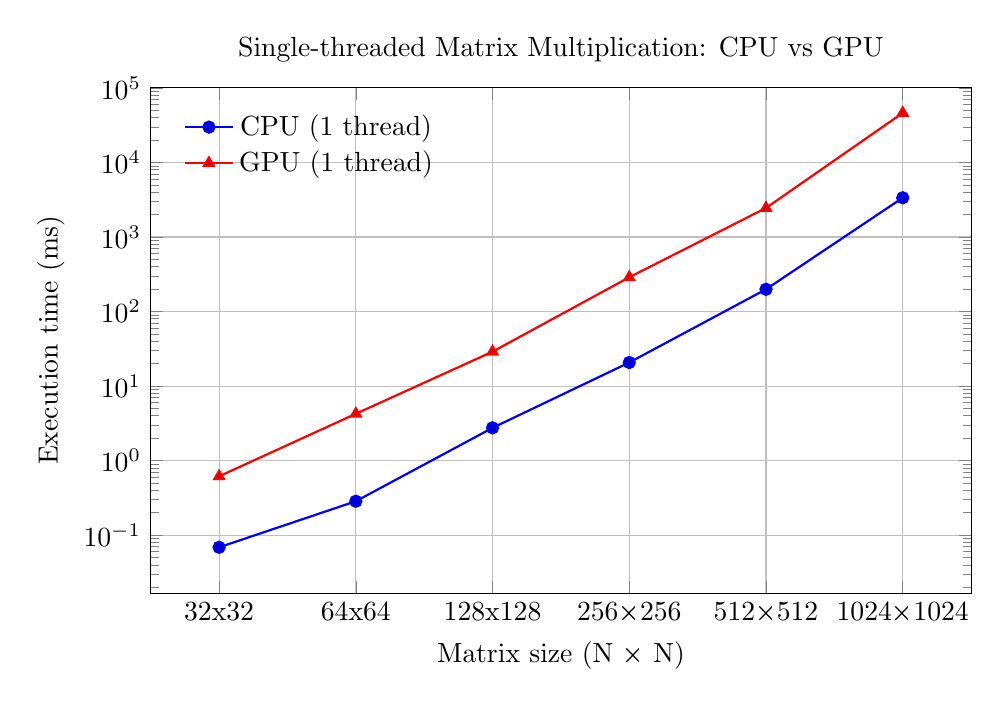
\begin{tikzpicture}
\begin{axis}[
    ymode=log,
    log basis y=10,
    width=12cm,
    height=8cm,
    xlabel={Matrix size (N × N)},
    ylabel={Execution time (ms)},
    title={Single-threaded Matrix Multiplication: CPU vs GPU},
    legend pos=north west,
    xtick=data,
    xticklabels={32x32, 64x64, 128x128, 256×256, 512×512, 1024×1024},
    ymin=0,
    ymax=100000,
    grid=major,
    legend style={draw=none, fill=none}
]

\addplot+[mark=*, thick, blue] coordinates {
    (1, 0.068705)
    (2, 0.285104)
    (3, 2.751817)
    (4, 20.706290)
    (5, 198.716200)
	(6, 3356.762000)
};
\addlegendentry{CPU (1 thread)}

\addplot+[mark=triangle*, thick, red] coordinates {
    (1, 0.615584)
    (2, 4.249685)
    (3, 28.923530)
    (4, 287.943700)
    (5, 2446.466000)
    (6, 46097.410000)
};
\addlegendentry{GPU (1 thread)}

\end{axis}
\end{tikzpicture}

  }
  \caption{Single threaded Matrix Multiplication Execution}
  \label{fig:singlethreadedgraph}
\end{figure}

\begin{figure}[htbp]
	\centering
	\resizebox{1.0\linewidth}{!}{
		\begin{tabular}{|r|r|r|r|r|}
\hline
\textbf{Matrix Size (n $\times$ n)} & \textbf{CPU Time (ms)} & \textbf{GPU Time (ms)} & \textbf{Speedup (GPU/CPU)} \\
\hline
32 $\times$ 32     & 0.068705   & 0.615584    & 11.970438 \\
64 $\times$ 64     & 0.285104   & 4.249685    & 15.554119 \\
128 $\times$ 128   & 2.751817   & 28.923530   & 11.419879 \\
256 $\times$ 256   & 20.706290  & 287.933700  & 13.906730 \\
512 $\times$ 512   & 198.716200 & 2446.466000 & 12.323010 \\
1024 $\times$ 1024 & 3356.762000 & 46097.410000 & 13.745850 \\
\hline
\end{tabular}


	}
	\caption{Data Matrix}
	\label{fig:singlethreadedmatrix}
\end{figure}	




\acsp{GPU} have revolutionized data processing and machine learning training and inference with their ability to handle massive amounts of data and execute simple, but highly-parallelized computations.
Data processing systems, based on traditional CPUs, rely on a \ac{MIMD} architecture that excels at handling complex control logic at high frequencies by executing different instructions on seperate data streams concurrently. 
However, for  tasks that require the repeated execution of singular instructions such as large-scale data processing workloads, \acsp{CPU} are burdened by the overhead of the complex control logic, where a simpler, more parallel design would be more effective.
\acs{GPU}s, created to overcome this limitation, use a \ac{SIMT} architecture with thousands of simpler, but slower threads executing simultaneously. 
% TODO
For example, the current architecture generally supports as many as 2048 threads in a single block, which can run on a single \ac{SM}, scaling the number of concurrent threads by the number of \acsp{SM}, by the number of \acsp{SM}, 80 on the newer models. 
% TODO
The parallelism provided by the \ac{SIMT} model allows a far higher throughput that outperforms \acsp{CPU}. 
Here, each data element is processed by its own thread, allowing the same instruction to be executed simultaneously across numerous data streams.

% TODO
Real time systems, which rely extensively on machine learning tasks and data processing tasks, Higher data processing performance is vital to autonomous systems, which rely extensively on machine learning tasks and sensor data processing. 
In autonomous systems a multitude of modules require deep learning, a machine learning technique, to automatically extract patterns, such as computer vision, and make decisions \cite{JEON2021167}.
Deep learning, inspired by the structure of the human brain, is composed of layers of numerous interconnected, identical nodes called neural networks.  
Neural network models rely on mathematical operations between different neighboring layers to perform inference, essentially the prediction making or recognition process.
The layers are represented as matrices, which then get multiplied and convoluted with one another and are used by specialized functions, called activation functions, to introduce non-linearity. 
With very large neural networks with thousands or millions of nodes, the inference computation is repetitive and slow. 
The capability to execute these repeptitive workloads concurrently across different dataset makes \acsp{GPU} fundamental to performance in tasks using complex neural networks.  
Furthermore, \acsp{GPU} are necessary to process the data rate produced by high-bandwidth, high-frequency sensors used in autonomous driving. 
The parallelism in \acs{GPU}s makes them the ideal platform over CPUs for deep learning and data processing tasks, tasks fundamental for autonomous driving systems.


Real time systems, such as autonomous driving, are designed with strict timing constraints in mind, to ensure predictable and deterministic behavior \cite{10155700}. 
deadlines, which are subdivided into soft and hard-deadlines. 
Hard deadlines are critical and a failure leads to the systems failure or unsafe conditions. 
For example, in autonomous driving, collision avoidance with another vehicle and brake activation are hard deadlines. 
If these deadlines are not met, the safety of the passengers and the system is at risk. 
On the other hand, soft deadlines are not critical and missing these deadlines degrades performance, but does not cause system failure. 
In autonomous driving, this would show in route planning and navigation updates, where a delay would lead to suboptimal paths, but safety is not comprimised. 
Real time systems need to be capable of effectively and efficiently switching from lower priority tasks, soft deadline tasks, to high priority, hard deadline tasks, to ensure the safety both for the passengers and nearby individuals.  





\subsection{Necessesity of \acsp{GPU} in Autonomous Driving}

\subsection{Autonomous Driving as a Real Time System}

\section{Background}
\subsection{Asynchronous Programming and Coroutines}

Asynchronous programming is a method of programming a system to handle tasks concurrently instead of sequentially. 
Typically used in conjunction with tasks that delay or have high wait-times, such as I/O heavy jobs, asynchronous programming reduces overall execution time by more efficiently using processing ressources. 
For example, while waiting for I/O heavy input like sensor I/O, asynchronous code lets other tasks execute in the meantime, before returning when the data arrives.  
For real-time systems, asynchronous programming additionally uses the intermittant execution model to enforce determinism. 
By allowing the \acsp{GPU} to switch between concurrent tasks, hard deadlines can be immediately enforced without delay. 


Coroutines, an implementation of asynchronous programming, uses suspendable functions to halt execution. 
Suspendable functions are implemented by capturing the current context, know as the continuation, of the currently running thread and save the data to be run later \cite{Zheng2022LuisaRender}. 
After being saved, a new process can take over execution, without interrupting or overwritting the state of the previous process. 
Once the intermittant process or higher priority process has finished execution, the original task can continue executing by restoring the process context, which was previously saved. 
Capturing the continuation of a function allows the resumption of the program to be strategically deferred. 

%Here, the scheduled tasks are independent of the control flow, meaning the execution order of the subtasks





\subsection{NVIDIA Tesla V100 Architecture}

For the purpose of this thesis, the NVIDIA Tesla V100 accelerator, which uses the Volta GV100 \ac{GPU} architecture, was selected due to its availability and high-performance computing capabilities.
At the core of its execution model is the warp, a group of 32 threads executing in \ac{SIMT} fashion \cite{nvidia2017tesla}.
Each warp is scheduled and dispatched within one of the 4 processing partitions of a \ac{SM}. 
The warp scheduler and warp dispatcher each handle 32 threads per clock cycle. 
Within each \ac{SM} partition, there are Tensor Cores for deep learning, 64 bit-\ac{FP} cores, \ac{LD/ST} units, a register file, and \acs{SFU}s for mathematical functions such as  sine and square root. 
Additionally, each partition contains 16 Cuda cores, which can execute both \ac{FP} 32 bit and \ac{INT} 32 bit instructions, but not simultaneously. 
Each partition has its own L0 instruction cache, while all partitions share a L1 instruction and data cache. 
A \ac{SM} can support up to 64 concurrent warps, allowing a maximum of $64 * 32 = 2048$ threads per \ac{SM}. 
At a higher level, two \acs{SM}s are grouped to form a \ac{TPC}. 
The Tesla V100 GPU consists of six \acs{GPC}s, each containing seven \acs{TPC}s, resulting in a total of 84 \acs{SM}s across the chip. 
This hierarchical organization, from warps to \acs{SM}s, \acs{TPC}s, and \acs{GPC}s, enables the Tesla V100 to efficiently handle massively parallel workloads, making it well-suited for high-performance computing and deel learning applications. 

 %\section{Motivation}
 %In autonomous driving and other real time system tasks, GPUs are essential for data processing and machine learning; however,  existing GPU scheduling techniques fail to meet the strict timing requirements of real-time applications.
 %GPU tasks are traditional queued and scheduled based on availabilty to optimize for high throughput applications like graphics rendering and offline machine learning training.
 %These tasks run to completion before switching tasks, meaning multiple tasks, such as the different modules in autonomous driving cannot efficiently share resources. 
 %Depending on the current workload for the GPU, execution times and latency can vary. 
 %These limitations make existing GPU scheduling mechanisms unsuitable for real-time applications like autonomous driving, where deadlines need to be met to ensure the safety of the system and passengers. 

%Citation test~\parencite{latex}.

%Acronyms must be added in \texttt{main.tex} and are referenced using macros. The first occurrence is automatically replaced with the long version of the acronym, while all subsequent usages use the abbreviation.

%E.g. \texttt{\textbackslash ac\{TUM\}, \textbackslash ac\{TUM\}} $\Rightarrow$ \ac{TUM}, \ac{TUM}

%For more details, see the documentation of the \texttt{acronym} package\footnote{\url{https://ctan.org/pkg/acronym}}.




%Autonomous driving system

%In order to react in time to input, autonomous driving systems need to efficiently process 

%By removing human error and utilizing the faster reaction times of computers, autonomous driving can make transportation safer, more accessible, improve traffic efficiency, and reduce the number of traffic accidents.

%For \ac{AVs}, driving tasks rely on complex computations to both understand the surrounding environment and to react to it in real-time.
%Many of these computations are scheduled onto a \ac{\ac{GPU}}, to leverage the high degree of parallelism in the architecture. 
%However, similar to \ac{CPU}s, the \ac{\ac{GPU}} can experience contention when multiple tasks compete for processing power. 
%Unlike \ac{CPU}s, though, \ac{\ac{GPU}}s are less efficient at quickly switching between different tasks, which can lead to delays and unpredictability. 
%If too many tasks get scheduled at once, the system's ability to meet critical deadlines can be comprimised, potentially leading to safety hazards. 
%Using coroutines on persistant threads, \ac{\ac{GPU}} scheduling can be adapted to mitigate contention and ensure real-time system guarantees, enhancing the safety and reliability of \ac{AV}s.


%These autonomous driving modules use vast amounts of data for their computation tasks, which are based in deep learning, a machine learning technique that demands vast amounts of computational resources.
%Deep learning, inspired by the structure of the human brain, utilizes neural networks, with many layers of neural nodes, to automatically extract patterns, enabling decision-making tasks such as classification and object detection.  
%In perception, deep learning models, particularily \acs{CNN}s identify objects, lane markings, pedestrians, vehicles, and traffic lights from the raw sensor data. 
%Beyond perception, deep learning enhances localization by refining sensor fusion techniques, improving accuracy in determining the vehicles position. 
%Furthermore, deep learning also supports planning and control, through reinforcement learning and predictive models to optimize trajectories. 
%The real-time nature of these components are needed to reduce the latency, which requires these models to continously be updating their predictions as new sensor input arrives and the vehicle moves.
%This places a high demand on the hardware, requiring high-performance accelerators to process vast amounts of data efficiently. 
%To meet these requirements, these computations are scheduled on to a \ac{GPU}, which provides the high degree of parallelism required by the vast amount of data and computations within autonomous driving. 
